\section{Introducción}
	\subsection{Motivación}
	En el vertiginoso avance de la tecnología, la aplicación de redes neuronales en el procesamiento de imágenes ha emergido como un catalizador revolucionario en diversas disciplinas. Entre las múltiples facetas que abarca esta amalgama de inteligencia artificial y visión computarizada, la detección y clasificación de señales de tránsito se destaca como un campo de estudio de gran relevancia e impacto práctico.
La seguridad vial es una preocupación global de suma importancia, y el tráfico vehicular se presenta como un escenario dinámico y complejo donde la correcta interpretación de señales juega un papel crucial. La detección automatizada y la clasificación precisa de señales de tránsito no solo pueden potenciar la eficiencia de los sistemas de transporte, sino que también desempeñan un papel esencial en la prevención de accidentes y la mejora de la movilidad urbana.
	\begin{figure}[ht]
		\centering
		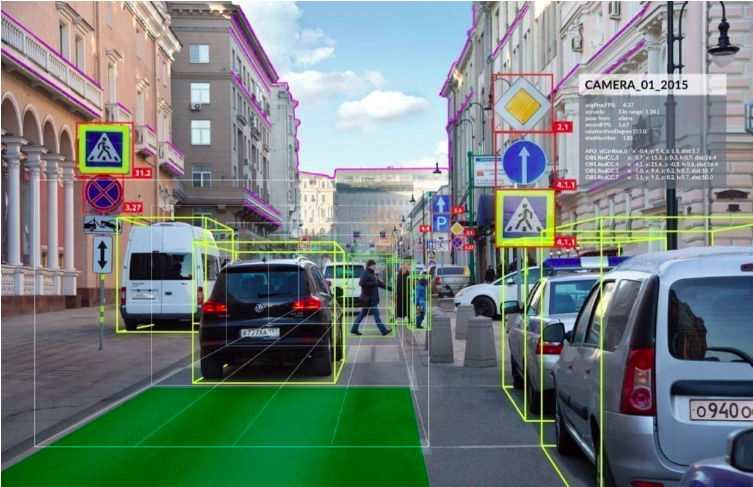
\includegraphics[height=7cm]{3}
		\caption{Reconocimiento de Objetos.}
	\end{figure}
	
El crecimiento exponencial de datos visuales en entornos urbanos y la necesidad de respuestas rápidas ante señales cambiantes hacen imperativa la adopción de enfoques avanzados. Acá es donde las redes neuronales toman importancia, porque su capacidad para aprender patrones complejos a partir de grandes conjuntos de datos permite el desarrollo de modelos capaces de discernir con precisión las señales de tráfico en imágenes, incluso en condiciones adversas.
En este contexto, la motivación subyacente es impulsar la aplicación de redes neuronales en el ámbito específico de la detección y clasificación de señales de tránsito.

\subsection {Objetivo}
\clearpage

\section{Marco Teórico}
	\subsection{Detección de Objetos}
	La detección de objetos constituye una rama esencial en el campo del procesamiento de imágenes y la visión por computadora. Su objetivo principal es discernir y localizar la presencia de uno o más objetos dentro de una imagen completa, asignándoles una identidad específica.
Las técnicas de detección de objetos se han desarrollado de manera significativa en respuesta a la creciente necesidad de sistemas capaces de comprender y responder a entornos visuales complejos. Uno de los enfoques más destacados y exitosos en este ámbito es el uso de redes neuronales convolucionales (CNN), que han demostrado una eficacia excepcional en la extracción de características relevantes de las imágenes.
La arquitectura típica para la detección de objetos a menudo involucra dos etapas cruciales: la generación de propuestas y la clasificación de esas propuestas. En la primera etapa, se utilizan técnicas como Region Proposal Networks (RPN) para proponer regiones de interés que podrían contener objetos. Posteriormente, estas regiones son clasificadas y refinadas utilizando capas de clasificación y regresión.

	\begin{figure}[ht]
	    \centering
		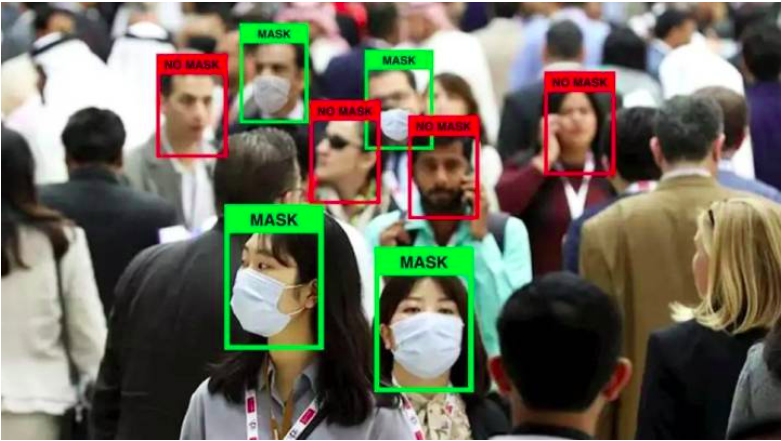
\includegraphics[scale=.4]{4}
		\caption{Reconocimiento facial}
	\end{figure}		
	
	Un enfoque más reciente y potente en la detección de objetos es la utilización de modelos de detección de objetos de una sola etapa, como YOLO (You Only Look Once) y SSD (Single Shot Multibox Detector). Estos modelos permiten la detección de objetos en tiempo real al abordar la tarea de manera conjunta, prediciendo las clases y las ubicaciones de los objetos de una sola vez.
Además, existen distintos tipos de detecciones y clasificaciones:
	\begin{itemize}
		\item Clasificación de la imagen.
		\item Clasificación con Localización.
		\item Detección.
	\end{itemize}

	\subsection{Clasificación de la imágen}
	En líneas generales, la clasificación de imágenes implica el uso de CNN seguidas de capas totalmente conectadas. Estas redes convolucionales son particularmente eficientes en la extracción de características relevantes, como bordes, texturas y patrones, mientras que las capas totalmente conectadas permiten la interpretación global de estas características para realizar la clasificación final.
Por ejemplo, en el contexto específico de la detección de vehículos, el objetivo de la clasificación se centraría en determinar la probabilidad de que la imagen contenga un automóvil. Esta probabilidad se obtiene al alimentar la imagen a través de la red neuronal, que ha sido previamente entrenada para reconocer patrones asociados con la presencia de vehículos.
	\begin{figure}[ht]
	    \centering
		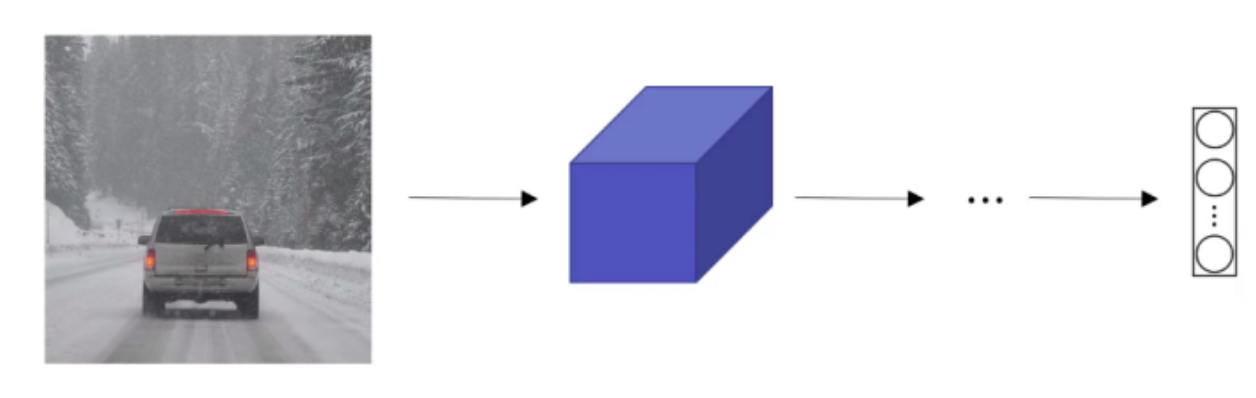
\includegraphics[scale=.30]{5}
		\caption{Representación del proceso de clasificación}
	\end{figure}

	\subsection{Clasificación con Localización}
	Para refinar aún más esta tarea, se pueden agregar neuronas de salida adicionales que proporcionen información sobre la localización del vehículo. Este enfoque, a menudo utilizado en sistemas de detección y clasificación de objetos, utiliza una bounding box (caja delimitadora) para representar la región en la que se encuentra el objeto de interés. En el caso de la detección de vehículos, esta \texttt{bounding box} se define mediante cuatro valores: \textbf{bx} (coordenada x del centro), \textbf{by} (coordenada y del centro), \textbf{bh} (altura) y \textbf{bw} (ancho)
	
	\begin{figure}[ht]
	    \centering
		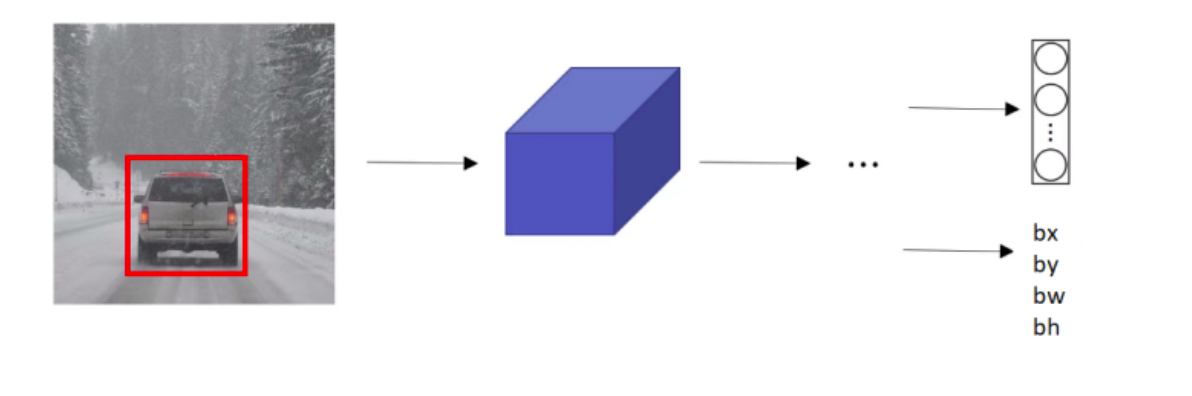
\includegraphics[scale=.35]{6}
		\caption{Representación del proceso de clasificación con localización}
	\end{figure}
	
	La inclusión de esta información espacial permite no solo identificar la presencia de un vehículo en la imagen, sino también delimitar su ubicación precisa. Este enfoque, combinado con técnicas avanzadas de clasificación, potencia la capacidad del sistema para comprender la escena visual en su totalidad y, en el caso específico de la detección de vehículos, proporcionar información detallada sobre su posición en la imagen.
	
	Por ejemplo, la salida de la red de clasificación con localización, considerando tres clases de objetos diferentes, sería la siguiente:
	
	\begin{center}
		\large{$y = [p_c$ $b_x$ $b_y$ $b_w$ $c_1$ $c_2$ $c_3]^T$}
	\end{center}
	
	Si ahora planteamos la función de pérdida de la salida (con MSE) tenemos:
	\vspace{0.3cm}
	\begin{itemize}[left=2cm]
	
	\item Si $p_c=1$
	\end{itemize}
	
	\begin{center}
		\large{$L(y,\hat{y}) = (\hat{y_1}-y_1)^2 + (\hat{y_2}-y_2)^2 +$ \dots $+ (\hat{y_8}-y_8)^2$}
	\end{center}	
		
	\begin{itemize}[left=2cm]
	\item Si $p_c=0$
	\end{itemize}
	
	\begin{center}
		\large{$L(y,\hat{y}) = (\hat{y_1}-y_1)^2$}
	\end{center}
	\pagebreak
	Por lo general se utiliza la función de pérdida log likelihood para las clases, mse para las coordenadas de la región limitante y logistic regression para $p_c$.

	\subsection{Redes STN}
	Las Redes STN, o Redes de Transformadores Espaciales (Spatial Transformer Networks), representan un enfoque innovador en el campo de las Redes Neuronales Convolucionales (CNN). Estas redes han sido diseñadas para abordar la invarianza espacial en las entradas, permitiendo que la red aprenda a manejar variaciones en rotación, traslación y escala de manera más efectiva.
	
	\vspace{0.3cm}
	\begin{figure}[ht]
	    \centering
		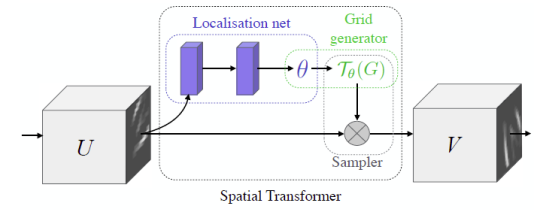
\includegraphics[scale=.5]{9}
		\caption{Representación de un Transformador espacial}
	\end{figure}
	\vspace{0.3cm}
	
	El núcleo distintivo de una Red STN radica en su incorporación de módulos de "transformadores espaciales". Estos módulos proporcionan a la red la capacidad de realizar transformaciones geométricas sobre las imágenes de entrada de manera automática durante el proceso de aprendizaje. Esta capacidad es fundamental para mejorar la robustez y la generalización del modelo, ya que permite que la red se vuelva espacialmente invariante a las variaciones mencionadas.
Las transformaciones espaciales, tales como rotaciones y traslaciones, pueden introducir variaciones significativas en las características visuales de una imagen. Por ejemplo, en el contexto de la detección de objetos en imágenes de tráfico, la rotación de una señal de tránsito o su traslación en la imagen pueden desafiar la capacidad de una red convencional para reconocerla de manera efectiva.
	
	\vspace{0.3cm}
	\begin{figure}[ht]
	    \centering
		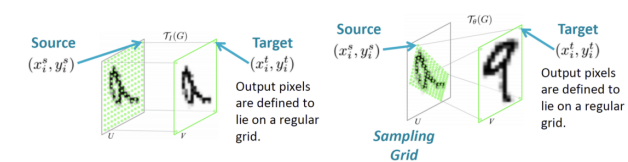
\includegraphics[scale=.5]{10}
		\caption{Representación de la aplicación de una transformación.}
	\end{figure}
	\vspace{0.3cm}

	Los módulos de transformadores espaciales en una Red STN actúan como mecanismos de atención, permitiendo a la red aprender a enfocarse en regiones específicas de la entrada y realizar ajustes geométricos según sea necesario. Esta adaptabilidad a las variaciones espaciales mejora la capacidad del modelo para capturar patrones relevantes independientemente de la orientación o posición en la imagen.
	
	Ahora bien, para el caso de una red de localización, donde se tiene un mapa de características de entrada U, con canales de ancho W y alto H, las salidas son  y los parámetros de transformación T, existiendo distintos tipos de transformaciones posibles. Una de esas transformaciones es la Transformación afín, donde dependiendo de los valores en la matriz, podemos transformar $(X_1, Y_1)$ a $(X_2, Y_2)$ con diferentes efectos.

	\begin{figure}[ht]
	    \centering
		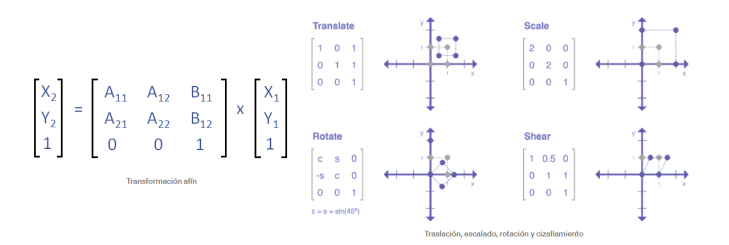
\includegraphics[scale=.5]{7}
		\caption{Representación de algunos efectos}
	\end{figure}
	

	




\section{Implementación}
\section{Resultados}
\section{Conclusión}
\section{Bibliografía}
